% Options for packages loaded elsewhere
\PassOptionsToPackage{unicode}{hyperref}
\PassOptionsToPackage{hyphens}{url}
\PassOptionsToPackage{dvipsnames,svgnames,x11names}{xcolor}
%
\documentclass[
  title=normal,
  notoc,
  bib=normal]{mnye}
\usepackage{amsmath,amssymb}
\usepackage{lmodern}
\usepackage{iftex}
\ifPDFTeX
  \usepackage[T1]{fontenc}
  \usepackage[utf8]{inputenc}
  \usepackage{textcomp} % provide euro and other symbols
\else % if luatex or xetex
  \usepackage{unicode-math}
  \defaultfontfeatures{Scale=MatchLowercase}
  \defaultfontfeatures[\rmfamily]{Ligatures=TeX,Scale=1}
\fi
% Use upquote if available, for straight quotes in verbatim environments
\IfFileExists{upquote.sty}{\usepackage{upquote}}{}
\IfFileExists{microtype.sty}{% use microtype if available
  \usepackage[]{microtype}
  \UseMicrotypeSet[protrusion]{basicmath} % disable protrusion for tt fonts
}{}
\makeatletter
\@ifundefined{KOMAClassName}{% if non-KOMA class
  \IfFileExists{parskip.sty}{%
    \usepackage{parskip}
  }{% else
    \setlength{\parindent}{0pt}
    \setlength{\parskip}{6pt plus 2pt minus 1pt}}
}{% if KOMA class
  \KOMAoptions{parskip=half}}
\makeatother
\usepackage{xcolor}
\IfFileExists{xurl.sty}{\usepackage{xurl}}{} % add URL line breaks if available
\IfFileExists{bookmark.sty}{\usepackage{bookmark}}{\usepackage{hyperref}}
\hypersetup{
  pdftitle={Ajuste de datos con R},
  pdfauthor={Eva María Mazcuñán Navarro},
  colorlinks=true,
  linkcolor={Maroon},
  filecolor={Maroon},
  citecolor={Blue},
  urlcolor={Blue},
  pdfcreator={LaTeX via pandoc}}
\urlstyle{same} % disable monospaced font for URLs
\usepackage{color}
\usepackage{fancyvrb}
\newcommand{\VerbBar}{|}
\newcommand{\VERB}{\Verb[commandchars=\\\{\}]}
\DefineVerbatimEnvironment{Highlighting}{Verbatim}{commandchars=\\\{\}}
% Add ',fontsize=\small' for more characters per line
\usepackage{framed}
\definecolor{shadecolor}{RGB}{248,248,248}
\newenvironment{Shaded}{\begin{snugshade}}{\end{snugshade}}
\newcommand{\AlertTok}[1]{\textcolor[rgb]{0.94,0.16,0.16}{#1}}
\newcommand{\AnnotationTok}[1]{\textcolor[rgb]{0.56,0.35,0.01}{\textbf{\textit{#1}}}}
\newcommand{\AttributeTok}[1]{\textcolor[rgb]{0.77,0.63,0.00}{#1}}
\newcommand{\BaseNTok}[1]{\textcolor[rgb]{0.00,0.00,0.81}{#1}}
\newcommand{\BuiltInTok}[1]{#1}
\newcommand{\CharTok}[1]{\textcolor[rgb]{0.31,0.60,0.02}{#1}}
\newcommand{\CommentTok}[1]{\textcolor[rgb]{0.56,0.35,0.01}{\textit{#1}}}
\newcommand{\CommentVarTok}[1]{\textcolor[rgb]{0.56,0.35,0.01}{\textbf{\textit{#1}}}}
\newcommand{\ConstantTok}[1]{\textcolor[rgb]{0.00,0.00,0.00}{#1}}
\newcommand{\ControlFlowTok}[1]{\textcolor[rgb]{0.13,0.29,0.53}{\textbf{#1}}}
\newcommand{\DataTypeTok}[1]{\textcolor[rgb]{0.13,0.29,0.53}{#1}}
\newcommand{\DecValTok}[1]{\textcolor[rgb]{0.00,0.00,0.81}{#1}}
\newcommand{\DocumentationTok}[1]{\textcolor[rgb]{0.56,0.35,0.01}{\textbf{\textit{#1}}}}
\newcommand{\ErrorTok}[1]{\textcolor[rgb]{0.64,0.00,0.00}{\textbf{#1}}}
\newcommand{\ExtensionTok}[1]{#1}
\newcommand{\FloatTok}[1]{\textcolor[rgb]{0.00,0.00,0.81}{#1}}
\newcommand{\FunctionTok}[1]{\textcolor[rgb]{0.00,0.00,0.00}{#1}}
\newcommand{\ImportTok}[1]{#1}
\newcommand{\InformationTok}[1]{\textcolor[rgb]{0.56,0.35,0.01}{\textbf{\textit{#1}}}}
\newcommand{\KeywordTok}[1]{\textcolor[rgb]{0.13,0.29,0.53}{\textbf{#1}}}
\newcommand{\NormalTok}[1]{#1}
\newcommand{\OperatorTok}[1]{\textcolor[rgb]{0.81,0.36,0.00}{\textbf{#1}}}
\newcommand{\OtherTok}[1]{\textcolor[rgb]{0.56,0.35,0.01}{#1}}
\newcommand{\PreprocessorTok}[1]{\textcolor[rgb]{0.56,0.35,0.01}{\textit{#1}}}
\newcommand{\RegionMarkerTok}[1]{#1}
\newcommand{\SpecialCharTok}[1]{\textcolor[rgb]{0.00,0.00,0.00}{#1}}
\newcommand{\SpecialStringTok}[1]{\textcolor[rgb]{0.31,0.60,0.02}{#1}}
\newcommand{\StringTok}[1]{\textcolor[rgb]{0.31,0.60,0.02}{#1}}
\newcommand{\VariableTok}[1]{\textcolor[rgb]{0.00,0.00,0.00}{#1}}
\newcommand{\VerbatimStringTok}[1]{\textcolor[rgb]{0.31,0.60,0.02}{#1}}
\newcommand{\WarningTok}[1]{\textcolor[rgb]{0.56,0.35,0.01}{\textbf{\textit{#1}}}}
\usepackage{longtable,booktabs,array}
\usepackage{calc} % for calculating minipage widths
% Correct order of tables after \paragraph or \subparagraph
\usepackage{etoolbox}
\makeatletter
\patchcmd\longtable{\par}{\if@noskipsec\mbox{}\fi\par}{}{}
\makeatother
% Allow footnotes in longtable head/foot
\IfFileExists{footnotehyper.sty}{\usepackage{footnotehyper}}{\usepackage{footnote}}
\makesavenoteenv{longtable}
\usepackage{graphicx}
\makeatletter
\def\maxwidth{\ifdim\Gin@nat@width>\linewidth\linewidth\else\Gin@nat@width\fi}
\def\maxheight{\ifdim\Gin@nat@height>\textheight\textheight\else\Gin@nat@height\fi}
\makeatother
% Scale images if necessary, so that they will not overflow the page
% margins by default, and it is still possible to overwrite the defaults
% using explicit options in \includegraphics[width, height, ...]{}
\setkeys{Gin}{width=\maxwidth,height=\maxheight,keepaspectratio}
% Set default figure placement to htbp
\makeatletter
\def\fps@figure{htbp}
\makeatother
\setlength{\emergencystretch}{3em} % prevent overfull lines
\providecommand{\tightlist}{%
  \setlength{\itemsep}{0pt}\setlength{\parskip}{0pt}}
\setcounter{secnumdepth}{5}
\usepackage{ehyperref}
\colorlet{etoccolor}{greenlink}
% This file is created the first time epdf_document is invoked
% but will not be overwriten afterwards.
%
% Preamble

\usepackage{ebox}
\usepackage{enotation}
\usepackage{fontawesome}

% https://stackoverflow.com/questions/63222203/rmarkdown-wrap-code-in-chunks-but-keep-breaks-after-pipe
\usepackage{fvextra}
\DefineVerbatimEnvironment{Highlighting}{Verbatim}{
    breaksymbolleft={},
    showspaces = false,
    showtabs = false,
    breaklines,
    commandchars=\\\{\}
}
% \lstset{
%   breaklines=true
% }

\pgfplotsset{compat=1.18}


\ifLuaTeX
  \usepackage{selnolig}  % disable illegal ligatures
\fi
\usepackage[]{biblatex}
\addbibresource{book.bib}
\addbibresource{packages.bib}

\title{Ajuste de datos con R}
\author{Eva María Mazcuñán Navarro}
\date{}

\begin{document}
\maketitle

% This file is created the first time epdf_document is invoked
% but will not be overwriten afterwards.
%
% Before Body

{
\hypersetup{linkcolor=etoccolor}
\setcounter{tocdepth}{2}
\tableofcontents
}
\hypertarget{section}{%
\section*{}\label{section}}

\hypertarget{intro}{%
\section*{Introducción}\label{intro}}
\addcontentsline{toc}{section}{Introducción}

En esta práctica estudiaremos cómo ajustar un modelo a un conjunto de datos experimentales, mediante la técnica de mínimos cuadrados, usando \textsf{R}.

Mientras que en los problemas que hemos a mano hasta ahora hemos considerado únicamente modelos lineales de uno o dos parámetros, en esta práctica consideraremos modelos tanto lineales como no lineales, y con un número arbitrario de parámetros. También podremos trabajar con un número de datos mucho más elevado que en los problemas resueltos a mano.

Seguiremos trabajando con una variable dependiente \(y\) y una única variable dependiente \(x\), aunque las técnicas que presentaremos se generalizan sin dificultad al caso de varias variables independientes.

\hypertarget{prerequisites}{%
\subsection*{Requisitos previos}\label{prerequisites}}
\addcontentsline{toc}{subsection}{Requisitos previos}

Antes de comenzar esta práctica, necesitas:

\begin{itemize}
\item
  Tener \textsf{R} y \textsf{RStudio} instalados en tu equipo (ver \href{https://emazcunan.github.io/install-r-rstudio/}{Instalación de R y RStudio}).
\item
  Haber estudiado la práctica \href{https://emazcunan.github.io/basics-r-rstudio/}{Primeros pasos con R y RStudio}.
\end{itemize}

\hypertarget{workflow}{%
\subsection*{Flujo de trabajo}\label{workflow}}
\addcontentsline{toc}{subsection}{Flujo de trabajo}

Documenta lo que vayas aprendiendo conforme leas la práctica usando un documento R Markdown. Puedes utilizar \href{https://drive.google.com/uc?id=1t9pjP_1Kjo8wgtav_I6hPHXxb5BqTIrc\&export=download}{esta plantilla}.

Se recomienda guardar el archivo R Markdown en una carpeta propia. En dicha carpeta se creará el archivo \textsf{HTML} resultante de la compilación y después añadiremos los archivos con los datos que usaremos a lo largo de la práctica.

Recuerda que para crear encabezados se utiliza la sintaxis \texttt{\#} (nivel 1), \texttt{\#\#} (nivel 2), \ldots; y que los bloques de código se crean con el atajo \texttt{Ctrl\ +\ Alt\ +\ I}.

Respecto al seccionado del documento, lo más práctico es que imites la estructura de este guión de prácticas.

\hypertarget{packages}{%
\section{Paquetes}\label{packages}}

Para utilizar las funciones que aparecerán a lo largo de la práctica empezamos cargando el paquete tidyverse:

\begin{Shaded}
\begin{Highlighting}[]
\FunctionTok{library}\NormalTok{(}\StringTok{"tidyverse"}\NormalTok{)}
\end{Highlighting}
\end{Shaded}

Aunque se puede cargar un paquete en cualquier punto de un documento R Markdown, se considera una buena práctica cargar todos los paquetes al inicio.

Así que, si a lo largo de la práctica fuera necesario cargar más paquetes, escribe la correspondiente instrucción para cargarlos con la función \VERB|\FunctionTok{library}\NormalTok{()}| al comienzo de tu documento, junto con esta primera instrucción.

\hypertarget{lm}{%
\section{Modelos lineales}\label{lm}}

Como hemos visto en teoría, dada una variable dependiente \(y\) y una variable independiente \(x\), un modelo lineal de parámetros \(\beta_1\), \(\beta_2\), \ldots{} \(\beta_p\) tiene la forma

\[
y = \beta_1 f_1(x) + \beta_2 f_2(x) + \dots +\beta_p f_p(x),
\]
siendo \(f_1\), \(f_2\), \(\dots\), \(f_p\) funciones conocidas.

En este capítulo veremos cómo ajustar este tipo de modelos para un conjunto observaciones usando la función \VERB|\FunctionTok{lm}\NormalTok{()}| (\textbf{l}inear \textbf{m}odel) de \textsf{R}.

Veremos también cómo representar gráficamente un ajuste usando la función \VERB|\FunctionTok{geom\_smooth}\NormalTok{()}| del paquete \texttt{ggplot2}.

\hypertarget{planteamiento-del-problema-el-prisma-de-vidrio}{%
\subsection{Planteamiento del problema: El prisma de vidrio}\label{planteamiento-del-problema-el-prisma-de-vidrio}}

Newton demostró con el prisma que la luz blanca es una mezcla de varios colores y que la refracción depende del color (longitud de onda).

En un experimento, se eligieron diferentes longitudes de onda \(\lambda\) y se trazó el camino seguido por el rayo de luz que atraviesa el prisma, midiendo el ángulo de desviación para, a partir del mismo, calcular el índice de refracción \(n\) del vidrio para el color seleccionado.

Los datos obtenidos se recogen en el archivo \href{https://drive.google.com/uc?export=download\&id=1fI5_KZA8MAiZVegFmtlQ7Cm4IzlGDQtg}{\texttt{refraction.csv}}(click para descargar), que contiene las variables:

\begin{itemize}
\item
  \texttt{lambda}: longitud de onda \(\lambda\), medida en \(nm\).
\item
  \texttt{n}: índice de refracción.
\end{itemize}

Descarga el fichero \texttt{refraction.csv} y guárdalo en una carpeta de nombre \texttt{data} dentro de tu directorio de trabajo.

Importamos los datos con \VERB|\FunctionTok{read\_csv}\NormalTok{()}| y los guardamos en un objeto de nombre \texttt{refraction}:

\begin{Shaded}
\begin{Highlighting}[]
\NormalTok{refraction }\OtherTok{\textless{}{-}} \FunctionTok{read\_csv}\NormalTok{(}\StringTok{"data/refraction.csv"}\NormalTok{)}
\end{Highlighting}
\end{Shaded}

Visualizamos los datos dibujando la nube de puntos \((\lambda, n)\) con \VERB|\FunctionTok{geom\_point}\NormalTok{()}|:

\begin{Shaded}
\begin{Highlighting}[]
\FunctionTok{ggplot}\NormalTok{(}
  \AttributeTok{data =}\NormalTok{ refraction,}
  \AttributeTok{mapping =} \FunctionTok{aes}\NormalTok{(}\AttributeTok{x =}\NormalTok{ lambda, }\AttributeTok{y =}\NormalTok{ n)}
\NormalTok{) }\SpecialCharTok{+}
  \FunctionTok{geom\_point}\NormalTok{()}
\end{Highlighting}
\end{Shaded}

\begin{center}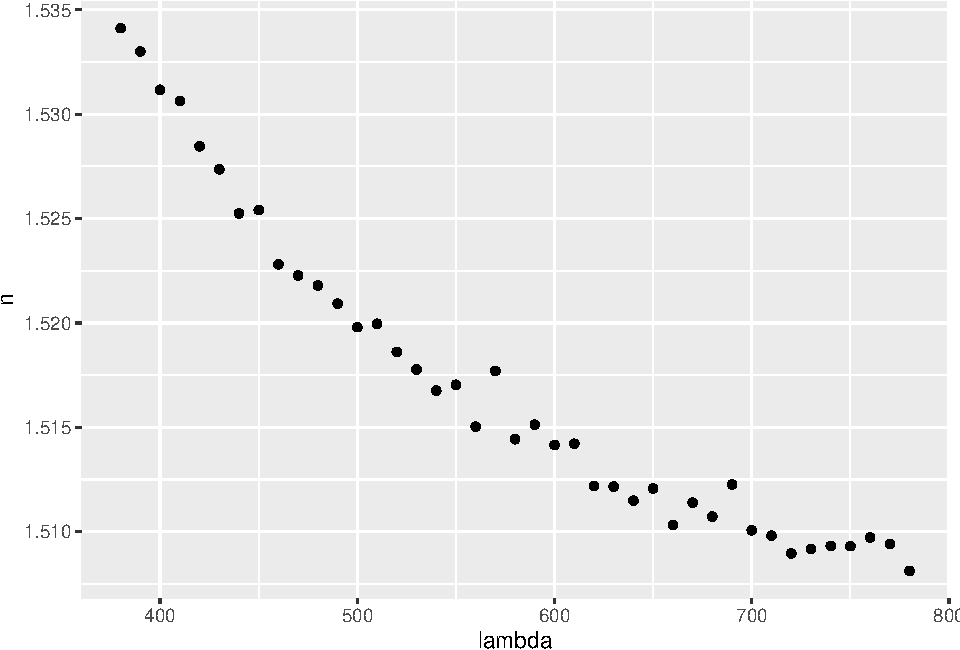
\includegraphics[width=1\linewidth]{fitting_files/figure-latex/unnamed-chunk-5-1} \end{center}

\hypertarget{ajuste-con-lm}{%
\subsection{\texorpdfstring{Ajuste con \texttt{lm()}}{Ajuste con lm()}}\label{ajuste-con-lm}}

Tomaremos como modelo la fórmula de Cauchy para los índices de refracción \(n\) en la región visible del espectro de longitud de onda \(\lambda\):
\[n(\lambda) = \beta_1 + \frac{\beta_2}{\lambda^2} + \frac{\beta_3}{\lambda^4}\]
donde \(\beta_1\), \(\beta_2\) y \(\beta_3\) son los parámetros a ajustar.

Como se indicó antes, la función de \textsf{R} para ajustar modelos lineales es \VERB|\FunctionTok{lm}\NormalTok{()}|. En la siguiente instrucción se utiliza la función \VERB|\FunctionTok{lm}\NormalTok{()}| para ajustar el modelo propuesto a las observaciones de nuestra hoja de datos, y se guarda el resultado en un objeto de nombre \texttt{fit\_cauchy}:

\begin{Shaded}
\begin{Highlighting}[]
\NormalTok{fit\_cauchy }\OtherTok{\textless{}{-}} \FunctionTok{lm}\NormalTok{(}
  \AttributeTok{data =}\NormalTok{ refraction,}
  \AttributeTok{formula =}\NormalTok{ n }\SpecialCharTok{\textasciitilde{}} \FunctionTok{I}\NormalTok{(}\DecValTok{1} \SpecialCharTok{/}\NormalTok{ lambda}\SpecialCharTok{\^{}}\DecValTok{2}\NormalTok{) }\SpecialCharTok{+} \FunctionTok{I}\NormalTok{(}\DecValTok{1} \SpecialCharTok{/}\NormalTok{ lambda}\SpecialCharTok{\^{}}\DecValTok{4}\NormalTok{)}
\NormalTok{)}
\end{Highlighting}
\end{Shaded}

En el código anterior, hemos usado los argumentos \texttt{data}, para especificar la hoja de datos con las observaciones, y \texttt{formula}, para indicar la fórmula del modelo (enseguida explicaremos cómo construir esta fórmula).

El resultado se almacena en un objeto de nombre \texttt{fit\_cauchy}.

Si imprimimos el objeto \texttt{fit\_cauchy} veremos los coeficientes del ajuste:

\begin{Shaded}
\begin{Highlighting}[]
\NormalTok{fit\_cauchy}
\end{Highlighting}
\end{Shaded}

\begin{Shaded}
\begin{Highlighting}[]
\NormalTok{\#\# }
\NormalTok{\#\# Call:}
\NormalTok{\#\# lm(formula = n \textasciitilde{} I(1/lambda\^{}2) + I(1/lambda\^{}4), data = refraction)}
\NormalTok{\#\# }
\NormalTok{\#\# Coefficients:}
\NormalTok{\#\#   (Intercept)  I(1/lambda\^{}2)  I(1/lambda\^{}4)  }
\NormalTok{\#\#           1.5         4908.3      7078041.7}
\end{Highlighting}
\end{Shaded}

La instrucción \VERB|\FunctionTok{summary}\NormalTok{(fit\_cauchy)}| revela que el objeto \texttt{fit\_cauchy} contiene mucha más información de la que muestra su simple impresión:

\begin{Shaded}
\begin{Highlighting}[]
\FunctionTok{summary}\NormalTok{(fit\_cauchy)}
\end{Highlighting}
\end{Shaded}

\begin{Shaded}
\begin{Highlighting}[]
\NormalTok{\#\# }
\NormalTok{\#\# Call:}
\NormalTok{\#\# lm(formula = n \textasciitilde{} I(1/lambda\^{}2) + I(1/lambda\^{}4), data = refraction)}
\NormalTok{\#\# }
\NormalTok{\#\# Residuals:}
\NormalTok{\#\#        Min         1Q     Median         3Q        Max }
\NormalTok{\#\# {-}1.294e{-}03 {-}4.672e{-}04  1.711e{-}05  2.982e{-}04  2.216e{-}03 }
\NormalTok{\#\# }
\NormalTok{\#\# Coefficients:}
\NormalTok{\#\#                Estimate Std. Error  t value Pr(\textgreater{}|t|)    }
\NormalTok{\#\# (Intercept)   1.500e+00  7.676e{-}04 1954.496  \textless{} 2e{-}16 ***}
\NormalTok{\#\# I(1/lambda\^{}2) 4.908e+03  4.342e+02   11.303 1.02e{-}13 ***}
\NormalTok{\#\# I(1/lambda\^{}4) 7.078e+06  5.376e+07    0.132    0.896    }
\NormalTok{\#\# {-}{-}{-}}
\NormalTok{\#\# Signif. codes:  0 \textquotesingle{}***\textquotesingle{} 0.001 \textquotesingle{}**\textquotesingle{} 0.01 \textquotesingle{}*\textquotesingle{} 0.05 \textquotesingle{}.\textquotesingle{} 0.1 \textquotesingle{} \textquotesingle{} 1}
\NormalTok{\#\# }
\NormalTok{\#\# Residual standard error: 0.0007213 on 38 degrees of freedom}
\NormalTok{\#\# Multiple R{-}squared:  0.9912, Adjusted R{-}squared:  0.9907 }
\NormalTok{\#\# F{-}statistic:  2131 on 2 and 38 DF,  p{-}value: \textless{} 2.2e{-}16}
\end{Highlighting}
\end{Shaded}

Ésta es la razón por la que hemos creado el objeto \texttt{fit\_cauchy} para almacenar la salida de la función \VERB|\FunctionTok{lm}\NormalTok{()}|: lo usaremos en los siguientes apartados para extraer información del ajuste realizado.

\hypertarget{fuxf3rmulas-en-r}{%
\subsection{Fórmulas en R}\label{fuxf3rmulas-en-r}}

Al usar la función \VERB|\FunctionTok{lm}\NormalTok{()}|, hemos indicado el siguiente valor para el argumento \texttt{formula} :

\texttt{n\ \textasciitilde{}\ I(1/lambda\^{}2)\ +\ I(1/lambda\^{}4)}

La expresión anterior es un objeto de \textsf{R} de tipo \texttt{formula}, que se corresponde con la fórmula de Cauchy que estamos usando como módelo

\[n(\lambda) = \beta_1 + \frac{\beta_2}{\lambda^2} + \frac{\beta_3}{\lambda^4}.\]

En la siguiente tabla se muestran algunos ejemplos más de fórmulas en \textsf{R} correspondientes a diferentes modelos:

\begin{longtable}[]{@{}cc@{}}
\toprule
Modelo & \texttt{formula} \\
\midrule
\endhead
\(y=\beta_1+\beta_2x\) & \texttt{y\ \textasciitilde{}\ x} \\
\(y=\beta_1 x\) & \texttt{y\ \textasciitilde{}\ 0\ +\ x} \\
\(y=\beta_1 + \beta_2 x + \beta_3 x^2\) & \texttt{y\ \textasciitilde{}\ x\ +\ I(x\^{}2)} \\
\(y=\beta_1 \cos(x)+ \beta_2\sin(x)\) & \texttt{y\ \textasciitilde{}\ 0\ +\ I(cos(x))\ +\ I(sin(x))} \\
\bottomrule
\end{longtable}

Para especificar la fórmula de un modelo en \textsf{R} hay que tener en cuenta las siguientes reglas:

\begin{itemize}
\item
  Cada sumando en una fórmula de \textsf{R}, indica la función que multiplica a un parámetro em la fórmula del modelo. Así, el sumando \texttt{x} en una fórmula de \textsf{R} será un sumando de la forma \(\beta_ix\) en la fórmula matemática del modelo.
\item
  \textsf{R} añade siempre una constante como primer sumando de la fórmula del modelo (\(\beta_1\) en los ejemplos anteriores). Para evitar la inclusión automática de esa constante hay que escribir el sumando \texttt{0}. Así, la fórmula \texttt{y\ \textasciitilde{}\ x} se corresponde con \(y = \beta_1 + \beta_2x\); y si se quiere omitir la constante \(\beta_1\), se ha de escribir \texttt{y\ \textasciitilde{}\ 0\ +\ x}.
\item
  Las funciones que son una transformación de la variable independiente se han de escribir incluidas en la función identidad \texttt{I()}. Por ejemplo, un término de la forma \(\beta_i x^2\) en la fórmula de un modelo se escribe en \textsf{R} como \texttt{I(x\^{}2)}.
\end{itemize}

\hypertarget{coeficientes}{%
\subsection{Coeficientes}\label{coeficientes}}

Para obtener los coeficientes del ajuste usamos la función \VERB|\FunctionTok{coefficients}\NormalTok{()}|:

\begin{Shaded}
\begin{Highlighting}[]
\FunctionTok{coefficients}\NormalTok{(fit\_cauchy)}
\end{Highlighting}
\end{Shaded}

\begin{Shaded}
\begin{Highlighting}[]
\NormalTok{\#\#   (Intercept) I(1/lambda\^{}2) I(1/lambda\^{}4) }
\NormalTok{\#\#  1.500310e+00  4.908268e+03  7.078042e+06}
\end{Highlighting}
\end{Shaded}

La salida nos informa de que los coeficientes que solucionan el problema de mínimos cuadrados (ecuaciones normales de Gauss) son:
\[\hat{\beta_1} = 1.50031,\]
\[\hat{\beta_2} = 4908.268,\]
y
\[\hat{\beta_3} = 7078042.\]

\textbf{Nota:} Dependiendo de la configuración, los valores de la salida pueden aparecer en notación científica, simbolizando \texttt{e+00}, \texttt{e+03} y \texttt{e+06} que hay que multiplicar por \(10^0=1\), \(10^3=1000\) y \(10^6=1000000\) respectivamente.

Por tanto el ajuste buscado es
\[n(\lambda) = 1.50031 + \frac{4908.268}{\lambda^2} + \frac{7078042}{\lambda^4}.\]

\hypertarget{valores-ajustados}{%
\subsection{Valores ajustados}\label{valores-ajustados}}

Los valores ajustados (o esperados) para la variable dependiente se obtienen con la función \VERB|\FunctionTok{fitted}\NormalTok{()}|:

\begin{Shaded}
\begin{Highlighting}[]
\FunctionTok{fitted}\NormalTok{(fit\_cauchy)}
\end{Highlighting}
\end{Shaded}

\begin{Shaded}
\begin{Highlighting}[]
\NormalTok{\#\#        1        2        3        4        5        6        7        8 }
\NormalTok{\#\# 1.534640 1.532886 1.531263 1.529759 1.528362 1.527062 1.525851 1.524721 }
\NormalTok{\#\#        9       10       11       12       13       14       15       16 }
\NormalTok{\#\# 1.523664 1.522674 1.521746 1.520875 1.520056 1.519285 1.518558 1.517873 }
\NormalTok{\#\#       17       18       19       20       21       22       23       24 }
\NormalTok{\#\# 1.517225 1.516613 1.516033 1.515484 1.514963 1.514468 1.513998 1.513552 }
\NormalTok{\#\#       25       26       27       28       29       30       31       32 }
\NormalTok{\#\# 1.513126 1.512721 1.512335 1.511967 1.511615 1.511279 1.510958 1.510650 }
\NormalTok{\#\#       33       34       35       36       37       38       39       40 }
\NormalTok{\#\# 1.510356 1.510074 1.509804 1.509545 1.509297 1.509058 1.508829 1.508608 }
\NormalTok{\#\#       41 }
\NormalTok{\#\# 1.508396}
\end{Highlighting}
\end{Shaded}

\hypertarget{residuos}{%
\subsection{Residuos}\label{residuos}}

Para obtener los residuos del ajuste (\(\varepsilon_i\)) usamos la función \VERB|\FunctionTok{residuals}\NormalTok{()}|:

\begin{Shaded}
\begin{Highlighting}[]
\FunctionTok{residuals}\NormalTok{(fit\_cauchy)}
\end{Highlighting}
\end{Shaded}

\begin{Shaded}
\begin{Highlighting}[]
\NormalTok{\#\#             1             2             3             4             5 }
\NormalTok{\#\# {-}5.158258e{-}04  1.192086e{-}04 {-}9.157603e{-}05  8.724810e{-}04  9.998852e{-}05 }
\NormalTok{\#\#             6             7             8             9            10 }
\NormalTok{\#\#  2.981569e{-}04 {-}6.063847e{-}04  6.853349e{-}04 {-}8.594240e{-}04 {-}3.992586e{-}04 }
\NormalTok{\#\#            11            12            13            14            15 }
\NormalTok{\#\#  4.507231e{-}05  4.592263e{-}05 {-}2.575917e{-}04  6.782515e{-}04  5.616847e{-}05 }
\NormalTok{\#\#            16            17            18            19            20 }
\NormalTok{\#\# {-}1.021129e{-}04 {-}4.671765e{-}04  4.270844e{-}04 {-}1.002945e{-}03  2.215907e{-}03 }
\NormalTok{\#\#            21            22            23            24            25 }
\NormalTok{\#\# {-}5.376294e{-}04  6.594862e{-}04  1.524706e{-}04  6.591191e{-}04 {-}9.333365e{-}04 }
\NormalTok{\#\#            26            27            28            29            30 }
\NormalTok{\#\# {-}5.619564e{-}04 {-}8.481528e{-}04  9.871010e{-}05 {-}1.294146e{-}03  1.065956e{-}04 }
\NormalTok{\#\#            31            32            33            34            35 }
\NormalTok{\#\# {-}2.355407e{-}04  1.609116e{-}03 {-}2.899098e{-}04 {-}2.667854e{-}04 {-}8.491117e{-}04 }
\NormalTok{\#\#            36            37            38            39            40 }
\NormalTok{\#\# {-}3.842938e{-}04  1.710620e{-}05  2.483173e{-}04  8.932864e{-}04  7.950677e{-}04 }
\NormalTok{\#\#            41 }
\NormalTok{\#\# {-}2.796932e{-}04}
\end{Highlighting}
\end{Shaded}

Para calcular el error cuadrático del ajuste (\(RSS\)) usamos

\begin{Shaded}
\begin{Highlighting}[]
\FunctionTok{sum}\NormalTok{(}\FunctionTok{residuals}\NormalTok{(fit\_cauchy)}\SpecialCharTok{\^{}}\DecValTok{2}\NormalTok{)}
\end{Highlighting}
\end{Shaded}

\begin{Shaded}
\begin{Highlighting}[]
\NormalTok{\#\# [1] 1.976785e{-}05}
\end{Highlighting}
\end{Shaded}

En el resumen del ajuste podemos leer

\texttt{Residual\ standard\ error:\ 0.0007213\ on\ 38\ degrees\ of\ freedom}

El error estandard residual, que suele denotarse \(\sigma\), se obtiene con la función \VERB|\FunctionTok{sigma}\NormalTok{()}|.

\begin{Shaded}
\begin{Highlighting}[]
\FunctionTok{sigma}\NormalTok{(fit\_cauchy)}
\end{Highlighting}
\end{Shaded}

\begin{Shaded}
\begin{Highlighting}[]
\NormalTok{\#\# [1] 0.0007212534}
\end{Highlighting}
\end{Shaded}

La relación entre esta cantidad \(\sigma\) y el error cuadrático \(RSS\) es:
\[\sigma = \sqrt{RSS/38}\]
o equivalentemente
\[RSS=38\sigma^2.\]
El valor \(38\), se llama grados de libertad de los residuos y se obtiene de restar, a las \(n=41\) observaciones, los \(p=3\) parámetros del modelo. Se obtiene con la función \VERB|\FunctionTok{df.residual}\NormalTok{()}|. Comprobamos la relación entre el error residual estandar y \(RSS\):

\begin{Shaded}
\begin{Highlighting}[]
\FunctionTok{df.residual}\NormalTok{(fit\_cauchy) }\SpecialCharTok{*} \FunctionTok{sigma}\NormalTok{(fit\_cauchy)}\SpecialCharTok{\^{}}\DecValTok{2} \CommentTok{\# RSS}
\end{Highlighting}
\end{Shaded}

\begin{Shaded}
\begin{Highlighting}[]
\NormalTok{\#\# [1] 1.976785e{-}05}
\end{Highlighting}
\end{Shaded}

\hypertarget{predicciones}{%
\subsection{Predicciones}\label{predicciones}}

La siguiente tabla recoge las longitudes de onda correspondientes a algunos colores del arcoiris:

\begin{longtable}[]{@{}ll@{}}
\toprule
Color & \(\lambda\) \\
\midrule
\endhead
Rojo & 640 \\
Amarillo & 589 \\
Verde & 509 \\
Azul & 486 \\
Violeta & 434 \\
\bottomrule
\end{longtable}

Queremos calcular los índices de refracción que predice nuestro ajuste para los colores anteriores. Para hacerlo usamos la función \VERB|\FunctionTok{predict}\NormalTok{()}|:

\begin{Shaded}
\begin{Highlighting}[]
\CommentTok{\# hoja de datos con los nuevos valores de lambda}
\NormalTok{new\_lambda }\OtherTok{\textless{}{-}} \FunctionTok{tibble}\NormalTok{(}
  \AttributeTok{lambda =} \FunctionTok{c}\NormalTok{(}\DecValTok{640}\NormalTok{, }\DecValTok{589}\NormalTok{, }\DecValTok{509}\NormalTok{, }\DecValTok{486}\NormalTok{, }\DecValTok{434}\NormalTok{)}
\NormalTok{)}
\CommentTok{\# predicciones}
\FunctionTok{predict}\NormalTok{(}
\NormalTok{  fit\_cauchy,}
\NormalTok{  new\_lambda}
\NormalTok{)}
\end{Highlighting}
\end{Shaded}

\begin{Shaded}
\begin{Highlighting}[]
\NormalTok{\#\#        1        2        3        4        5 }
\NormalTok{\#\# 1.512335 1.514517 1.519360 1.521217 1.526568}
\end{Highlighting}
\end{Shaded}

En la función \VERB|\FunctionTok{predict}\NormalTok{()}| indicamos como primer argumento nuestro ajuste \texttt{fit\_cauchy} y como segundo argumento una hoja de datos, que hemos llamado \texttt{new\_lambda}, con los nuevos valores para la variable independiente \texttt{lambda}. Hemos construido dicha hoja de datos con la función \VERB|\FunctionTok{tibble}\NormalTok{()}| (\emph{tidy table}).

\hypertarget{gruxe1fico-del-ajuste}{%
\subsection{Gráfico del ajuste}\label{gruxe1fico-del-ajuste}}

Al comienzo del problema representamos la nube de puntos de nuestras observaciones con la función \VERB|\FunctionTok{geom\_point}\NormalTok{()}|. Añadimos ahora el gráfico del ajuste con la función \VERB|\FunctionTok{geom\_smooth}\NormalTok{()}|:

\begin{Shaded}
\begin{Highlighting}[]
\FunctionTok{ggplot}\NormalTok{(}
  \AttributeTok{data =}\NormalTok{ refraction,}
  \AttributeTok{mapping =} \FunctionTok{aes}\NormalTok{(}\AttributeTok{x =}\NormalTok{ lambda, }\AttributeTok{y =}\NormalTok{ n)}
\NormalTok{) }\SpecialCharTok{+}
  \FunctionTok{geom\_point}\NormalTok{() }\SpecialCharTok{+}
  \FunctionTok{geom\_smooth}\NormalTok{(}
    \AttributeTok{method =} \StringTok{"lm"}\NormalTok{,}
    \AttributeTok{formula =}\NormalTok{ y }\SpecialCharTok{\textasciitilde{}} \FunctionTok{I}\NormalTok{(}\DecValTok{1} \SpecialCharTok{/}\NormalTok{ x}\SpecialCharTok{\^{}}\DecValTok{2}\NormalTok{) }\SpecialCharTok{+} \FunctionTok{I}\NormalTok{(}\DecValTok{1} \SpecialCharTok{/}\NormalTok{ x}\SpecialCharTok{\^{}}\DecValTok{4}\NormalTok{),}
    \AttributeTok{se =} \ConstantTok{FALSE}
\NormalTok{  )}
\end{Highlighting}
\end{Shaded}

\begin{center}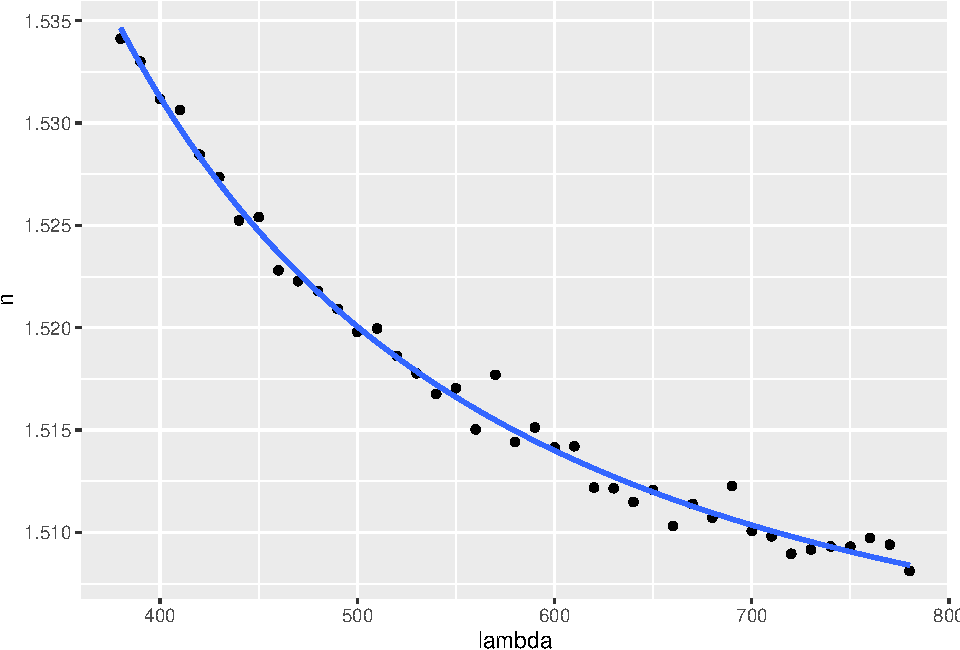
\includegraphics[width=1\linewidth]{fitting_files/figure-latex/unnamed-chunk-20-1} \end{center}

En los argumentos de \VERB|\FunctionTok{geom\_smooth}\NormalTok{()}| hemos escrito \VERB|\NormalTok{method }\OtherTok{=} \StringTok{"lm"}| para indicar que el ajuste se realiza con la función \VERB|\FunctionTok{lm}\NormalTok{()}|.

Notar que al especificar la fórmula del modelo en el argumento \texttt{formula} no se utilizan los nombres \texttt{lambda} y \texttt{n} de las variables --como se hizo en la función \VERB|\FunctionTok{lm}\NormalTok{()}|-- sino los nombres \texttt{x} e \texttt{y} de las estéticas asociadas.

El argumento \VERB|\NormalTok{se }\OtherTok{=} \ConstantTok{FALSE}| inhibe representar los intervalos de confianza (que estudiaremos en el último tema del curso).

\hypertarget{nls-tbc}{%
\section{Modelos no lineales}\label{nls-tbc}}

Modelos como
\[y = \beta_1 \beta_2^{x}\]
(modelo exponencial) o como
\[y = \beta_1x^{\beta_2}\]
(modelo potencial) no tienen una estructura lineal.

Para modelos lineales, el problema de encontrar los valores de los parámetros que minimizan el error cuadrático del ajuste se traduce en resolver el sistema de ecuaciones normales de Gauss, que es un sistema lineal.\\
Pero en el caso de modelos no lineales como los anteriores, la situación se complica porque ahora la solución viene dada por un sistema de ecuaciones no lineales.

En este capítulo veremos cómo ajustar este tipo de modelos a una colección de observaciones, usando la función \VERB|\FunctionTok{nls}\NormalTok{()}| (\textbf{n}onlinear \textbf{l}east \textbf{s}quares) de \textsf{R}.

\hypertarget{tbc}{%
\subsection{Continuará \ldots{}}\label{tbc}}

\printbibliography

% This file is created the first time epdf_document is invoked
% but will not be overwriten afterwards.
%
% After Body

\end{document}
